\documentclass{standalone}
\usepackage{tikz}
\usetikzlibrary{patterns, positioning}
\usepackage[sfdefault]{ClearSans} %% option 'sfdefault' activates Clear Sans as the default text font
\usepackage[T1]{fontenc}

\begin{document}
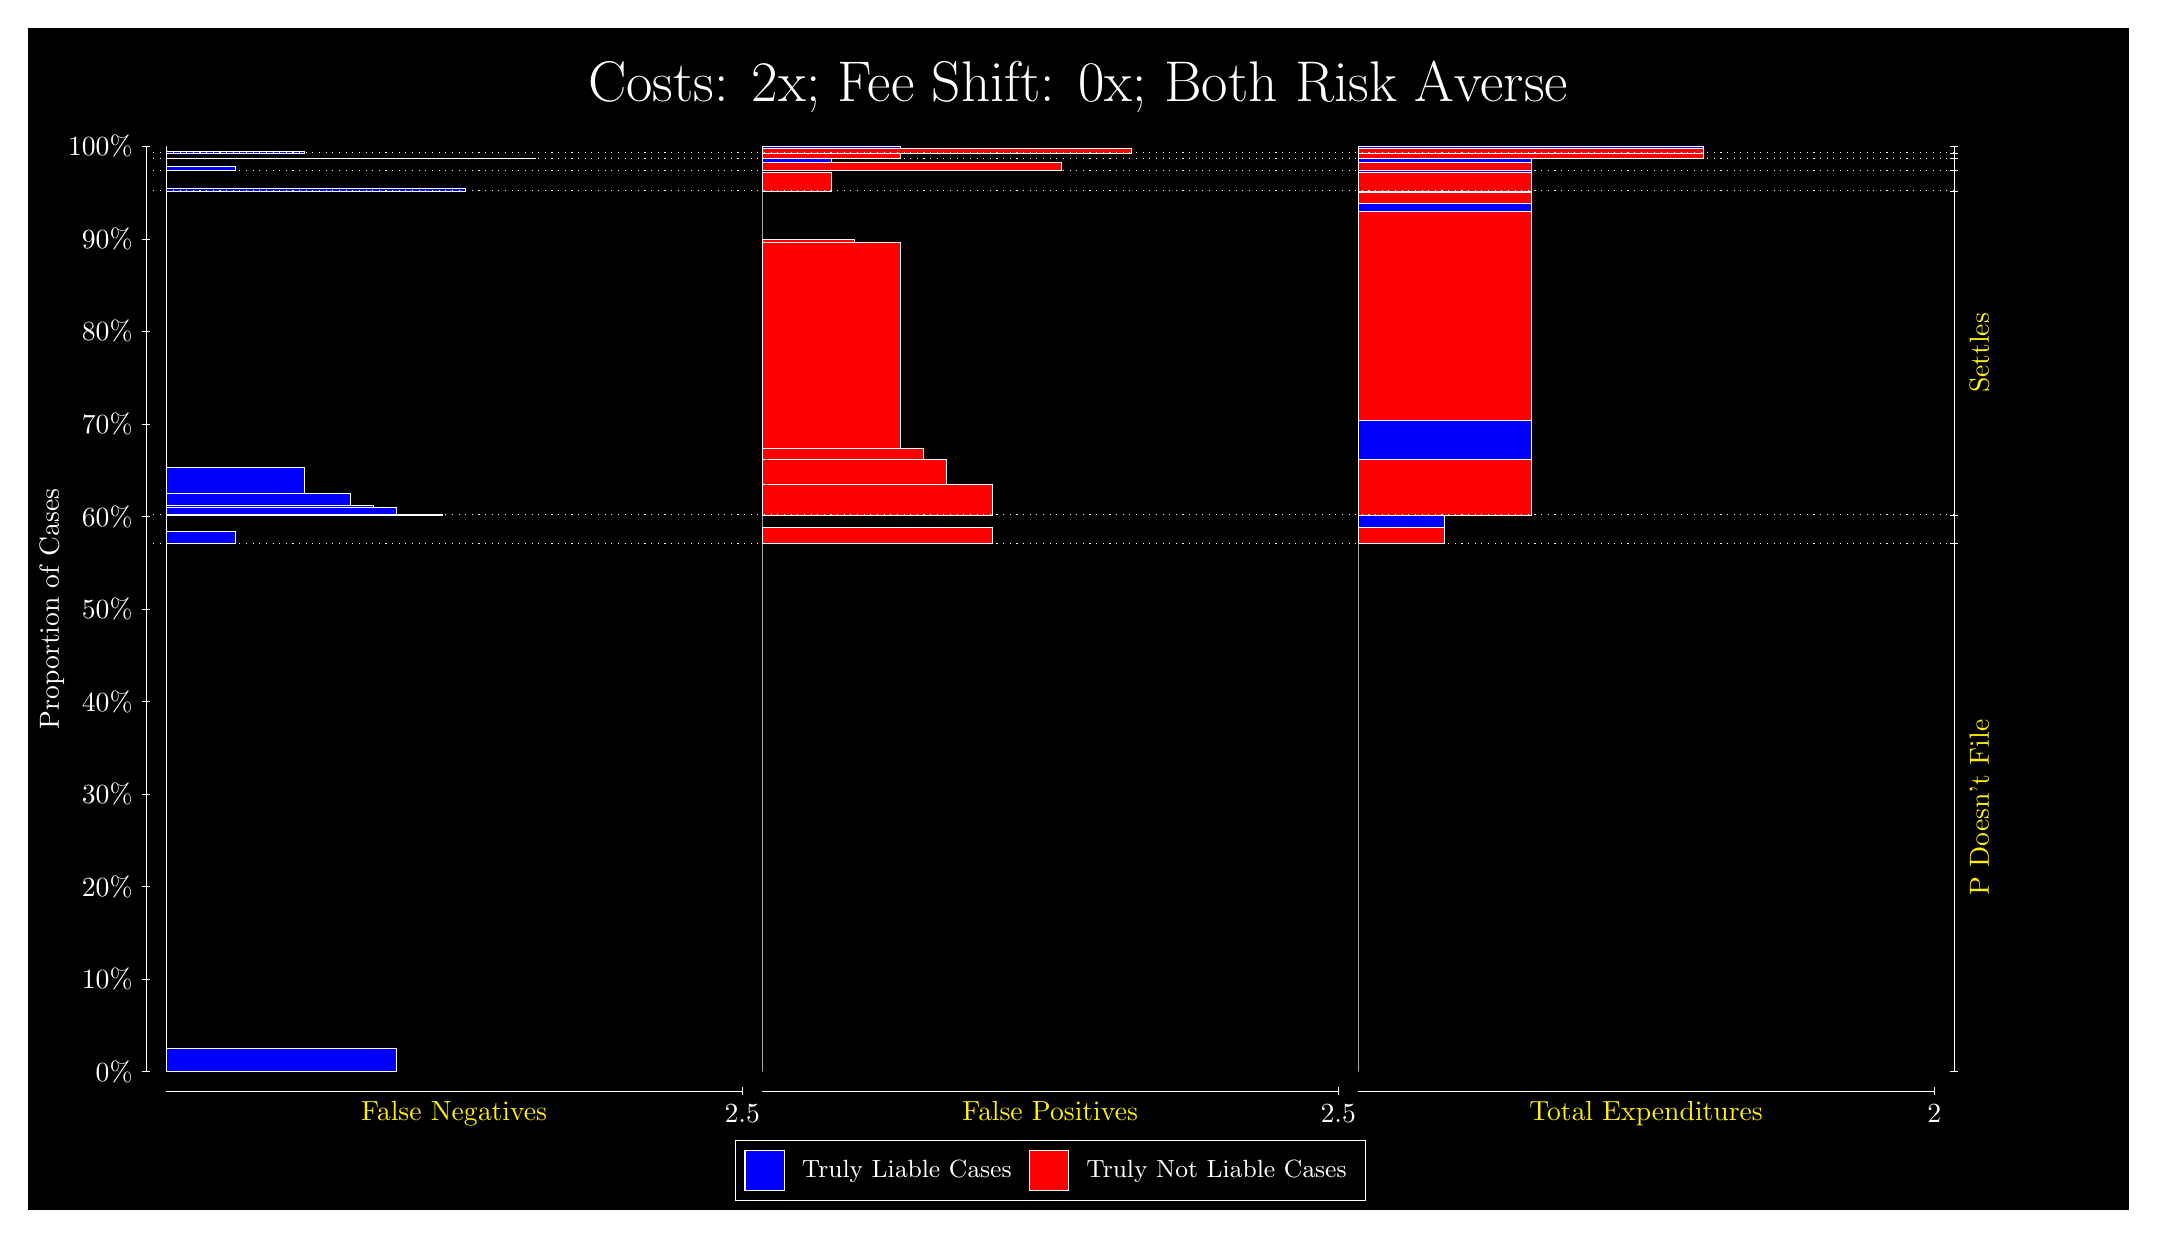
\begin{tikzpicture}
\draw[fill=black] (0,0) rectangle (26.667,15);
\draw[text=white] (0,13.5) rectangle (26.667,15) node[midway] {\huge Costs: 2x; Fee Shift: 0x; Both Risk Averse};
\draw[white, very thin] (1.5,1.75) -- (1.5,13.5);
\node[rotate=90, text=white, anchor=center] at (0.3, 7.625) {Proportion of Cases};
\draw[white, very thin] (1.45,1.75) -- (1.55,1.75);
\node[text=white, anchor=east] at (1.45, 1.75) {0\%};
\draw[white, very thin] (1.45,2.925) -- (1.55,2.925);
\node[text=white, anchor=east] at (1.45, 2.925) {10\%};
\draw[white, very thin] (1.45,4.1) -- (1.55,4.1);
\node[text=white, anchor=east] at (1.45, 4.1) {20\%};
\draw[white, very thin] (1.45,5.275) -- (1.55,5.275);
\node[text=white, anchor=east] at (1.45, 5.275) {30\%};
\draw[white, very thin] (1.45,6.45) -- (1.55,6.45);
\node[text=white, anchor=east] at (1.45, 6.45) {40\%};
\draw[white, very thin] (1.45,7.625) -- (1.55,7.625);
\node[text=white, anchor=east] at (1.45, 7.625) {50\%};
\draw[white, very thin] (1.45,8.8) -- (1.55,8.8);
\node[text=white, anchor=east] at (1.45, 8.8) {60\%};
\draw[white, very thin] (1.45,9.975) -- (1.55,9.975);
\node[text=white, anchor=east] at (1.45, 9.975) {70\%};
\draw[white, very thin] (1.45,11.15) -- (1.55,11.15);
\node[text=white, anchor=east] at (1.45, 11.15) {80\%};
\draw[white, very thin] (1.45,12.325) -- (1.55,12.325);
\node[text=white, anchor=east] at (1.45, 12.325) {90\%};
\draw[white, very thin] (1.45,13.5) -- (1.55,13.5);
\node[text=white, anchor=east] at (1.45, 13.5) {100\%};

\draw[white, very thin] (24.457,1.75) -- (24.457,13.5);
\draw[white, very thin] (24.407,1.75) -- (24.507,1.75);
\node[anchor=west] at (24.407, 1.75) {};
\draw[white, very thin] (24.407,8.4557) -- (24.507,8.4557);
\node[anchor=west] at (24.407, 8.4557) {};
\draw[white, very thin] (24.407,8.8189) -- (24.507,8.8189);
\node[anchor=west] at (24.407, 8.8189) {};
\draw[white, very thin] (24.407,12.935) -- (24.507,12.935);
\node[anchor=west] at (24.407, 12.935) {};
\draw[white, very thin] (24.407,13.198) -- (24.507,13.198);
\node[anchor=west] at (24.407, 13.198) {};
\draw[white, very thin] (24.407,13.343) -- (24.507,13.343);
\node[anchor=west] at (24.407, 13.343) {};
\draw[white, very thin] (24.407,13.418) -- (24.507,13.418);
\node[anchor=west] at (24.407, 13.418) {};
\draw[white, very thin] (24.407,13.5) -- (24.507,13.5);
\node[anchor=west] at (24.407, 13.5) {};

\draw[white, very thin, fill=blue] (1.75,1.75) rectangle (4.6775,2.0511);
\draw[white, very thin, fill=red] (1.75,2.0511) rectangle (1.75,8.4557);
\draw[white, very thin, fill=blue] (1.75,8.4557) rectangle (2.6283,8.6138);
\draw[white, very thin, fill=red] (1.75,8.6138) rectangle (1.75,8.8189);
\draw[white, very thin, fill=blue] (1.75,8.8189) rectangle (5.2631,8.824);
\draw[white, very thin, fill=blue] (1.75,8.824) rectangle (4.6775,8.9157);
\draw[white, very thin, fill=blue] (1.75,8.9157) rectangle (4.3848,8.9393);
\draw[white, very thin, fill=blue] (1.75,8.9393) rectangle (4.092,9.0928);
\draw[white, very thin, fill=blue] (1.75,9.0928) rectangle (3.5065,9.4301);
\draw[white, very thin, fill=red] (1.75,9.4301) rectangle (1.75,12.935);
\draw[white, very thin, fill=blue] (1.75,12.935) rectangle (5.5558,12.965);
\draw[white, very thin, fill=red] (1.75,12.965) rectangle (1.75,13.198);
\draw[white, very thin, fill=blue] (1.75,13.198) rectangle (2.6283,13.242);
\draw[white, very thin, fill=red] (1.75,13.242) rectangle (1.75,13.343);
\draw[white, very thin, fill=blue] (1.75,13.343) rectangle (6.4341,13.349);
\draw[white, very thin, fill=red] (1.75,13.349) rectangle (1.75,13.418);
\draw[white, very thin, fill=blue] (1.75,13.418) rectangle (3.5065,13.441);
\draw[white, very thin, fill=red] (1.75,13.441) rectangle (1.75,13.5);
\draw[white, very thin, fill=red] (9.3189,1.75) rectangle (9.3189,8.1546);
\draw[white, very thin, fill=blue] (9.3189,8.1546) rectangle (9.3189,8.4557);
\draw[white, very thin, fill=red] (9.3189,8.4557) rectangle (12.246,8.6608);
\draw[white, very thin, fill=blue] (9.3189,8.6608) rectangle (9.3189,8.8189);
\draw[white, very thin, fill=red] (9.3189,8.8189) rectangle (12.246,9.2098);
\draw[white, very thin, fill=red] (9.3189,9.2098) rectangle (11.661,9.5305);
\draw[white, very thin, fill=red] (9.3189,9.5305) rectangle (11.368,9.6636);
\draw[white, very thin, fill=red] (9.3189,9.6636) rectangle (11.075,12.278);
\draw[white, very thin, fill=red] (9.3189,12.278) rectangle (10.49,12.324);
\draw[white, very thin, fill=blue] (9.3189,12.324) rectangle (9.3189,12.935);
\draw[white, very thin, fill=red] (9.3189,12.935) rectangle (10.197,13.167);
\draw[white, very thin, fill=blue] (9.3189,13.167) rectangle (9.3189,13.198);
\draw[white, very thin, fill=red] (9.3189,13.198) rectangle (13.125,13.298);
\draw[white, very thin, fill=blue] (9.3189,13.298) rectangle (10.197,13.343);
\draw[white, very thin, fill=red] (9.3189,13.343) rectangle (11.075,13.411);
\draw[white, very thin, fill=blue] (9.3189,13.411) rectangle (9.3189,13.418);
\draw[white, very thin, fill=red] (9.3189,13.418) rectangle (14.003,13.477);
\draw[white, very thin, fill=blue] (9.3189,13.477) rectangle (11.075,13.5);
\draw[white, very thin, fill=red] (16.888,1.75) rectangle (16.888,8.1546);
\draw[white, very thin, fill=blue] (16.888,8.1546) rectangle (16.888,8.4557);
\draw[white, very thin, fill=red] (16.888,8.4557) rectangle (17.986,8.6608);
\draw[white, very thin, fill=blue] (16.888,8.6608) rectangle (17.986,8.8189);
\draw[white, very thin, fill=red] (16.888,8.8189) rectangle (19.083,9.5305);
\draw[white, very thin, fill=blue] (16.888,9.5305) rectangle (19.083,10.021);
\draw[white, very thin, fill=red] (16.888,10.021) rectangle (19.083,12.681);
\draw[white, very thin, fill=blue] (16.888,12.681) rectangle (19.083,12.778);
\draw[white, very thin, fill=red] (16.888,12.778) rectangle (19.083,12.911);
\draw[white, very thin, fill=blue] (16.888,12.911) rectangle (19.083,12.935);
\draw[white, very thin, fill=red] (16.888,12.935) rectangle (19.083,13.167);
\draw[white, very thin, fill=blue] (16.888,13.167) rectangle (19.083,13.198);
\draw[white, very thin, fill=red] (16.888,13.198) rectangle (19.083,13.298);
\draw[white, very thin, fill=blue] (16.888,13.298) rectangle (19.083,13.343);
\draw[white, very thin, fill=red] (16.888,13.343) rectangle (21.279,13.411);
\draw[white, very thin, fill=blue] (16.888,13.411) rectangle (21.279,13.418);
\draw[white, very thin, fill=red] (16.888,13.418) rectangle (21.279,13.477);
\draw[white, very thin, fill=blue] (16.888,13.477) rectangle (21.279,13.5);
\draw[white, dotted] (1.5,8.4557) -- (24.457,8.4557);
\draw[white, dotted] (1.5,8.8189) -- (24.457,8.8189);
\draw[white, dotted] (1.5,12.935) -- (24.457,12.935);
\draw[white, dotted] (1.5,13.198) -- (24.457,13.198);
\draw[white, dotted] (1.5,13.343) -- (24.457,13.343);
\draw[white, dotted] (1.5,13.418) -- (24.457,13.418);
\draw[white, very thin] (1.75,1.5) -- (9.0689,1.5);
\node[text=yellow, anchor=north] at (5.4094, 1.5) {False Negatives};
\draw[white, very thin] (9.0689,1.45) -- (9.0689,1.55);
\node[text=white, anchor=north] at (9.0689, 1.45) {2.5};

\draw[white, very thin] (9.3189,1.5) -- (16.638,1.5);
\node[text=yellow, anchor=north] at (12.978, 1.5) {False Positives};
\draw[white, very thin] (16.638,1.45) -- (16.638,1.55);
\node[text=white, anchor=north] at (16.638, 1.45) {2.5};

\draw[white, very thin] (16.888,1.5) -- (24.207,1.5);
\node[text=yellow, anchor=north] at (20.547, 1.5) {Total Expenditures};
\draw[white, very thin] (24.207,1.45) -- (24.207,1.55);
\node[text=white, anchor=north] at (24.207, 1.45) {2};

\node[text=yellow, centered, rotate=90] at (24.777, 5.1029) {P Doesn't File};

\node[text=yellow, centered, rotate=90] at (24.777, 10.877) {Settles};





\draw (12.978300999999998,1.5) node[draw=none] (baseCoordinate) {};
\begin{scope}[align=center]
        \matrix[scale=0.5, draw=white, below=0.5cm of baseCoordinate, nodes={draw}, column sep=0.1cm]{
            \node[rectangle, draw, minimum width=0.5cm, minimum height=0.5cm, fill=blue] {}; &
            \node[draw=none, font=\small, text=white] (B) {Truly Liable Cases}; &
            \node[rectangle, draw, minimum width=0.5cm, minimum height=0.5cm, fill=red] {}; &
            \node[draw=none, font=\small, text=white] (B) {Truly Not Liable Cases}; \\
            };
\end{scope}

\end{tikzpicture}
\end{document}